 \documentclass{report}
 
\usepackage[utf8]{inputenc} 
\usepackage[T1]{fontenc}      
\usepackage[top=2.0cm, bottom=3cm, left=3.0cm, right=3.0cm]{geometry}
\usepackage{graphicx}
\usepackage{wrapfig}
\usepackage{amsmath,esint }
\usepackage{amssymb}
\usepackage{esvect}
\graphicspath{{figures/}{../figures}}

\newcommand*\dif{\mathop{}\!\mathrm{d}}
\newcommand*\diver{\mathop{}\!\mathrm{div}}
\newcommand*\grad{\mathop{}\!\mathrm{grad}}

\begin{document}

\section*{Volatiles sur une ligne à haute tension}

L'étourneau sansonnet est une espèce d'oiseau sociale, se déplaçant par groupe de centaines, voire de milliers d'individus. On peut les apercevoir suspendus sur des lignes électriques avant leur envol. Pour notre étude, on peut modéliser l'étourneau comme une sphère de rayon $R=10$cm parfaitement conductrice (les tissus biologiques étant de bons conducteurs électriques). 

\begin{itemize}

	\item[$\bigvee$] Un étourneau se pose sur une ligne électrique au potentiel $V=50$kV. Quelle charge $Q$ va t-il porter à ce potentiel ? \textit{NB} : Les lignes électriques n'ont pas de revêtement isolant.
	
	\item[$\bigvee$] En réalité, la tension est alternative, à la fréquence $f=50$ Hz. Sachant que l'intensité létale est d'environ 10mA, l'étourneau prend-il un risque à se poser dessus ?
	
	\item[$\bigvee$] Un nuée de 1000 étourneaux se pose instantanément sur cette ligne électrique. Quelle va être la diminution de puissance électrique (temporaire) au bout de la ligne ?

\end{itemize} 

\newpage

\section*{\textit{Correction Volatiles sur une ligne à haute tension}}

\begin{itemize}

	\item[$\bigvee$] L'oiseau est une sphère de rayon $R$ portée au potentiel $V$ par rapport au sol, supposé très loin. Le potentiel est alors (à redémontrer par l'élève) :
	\begin{align*}
		V=\frac{Q}{4\pi\varepsilon_0 R}
	\end{align*}
	Il se charge donc d'une charge $Q=V\times 4\pi\varepsilon_0R=5,6\times10^{-7}$C.
	
	\item[$\bigvee$] Le courant étant alternatif, l'oiseau se charge et se décharge de $Q$ 50 fois par seconde. Il est donc parcouru par une intensité au minimum de $I=Qf=27\mu$A. On est loin du poulet rôti...
	
	\item[$\bigvee$] Lorsque les oiseaux se posent, il y a instantément une déviation de courant qui s'opèrent vers eux pour les monter à la charge $Q$. Il y a donc $N$ fois le courant $I$ qui est dévié le temps d'une période de charge, soit 27mA. Les ampérages circulant dans les lignes étant typiquement de l'ordre de l'ampère, on est loin d'avoir des problèmes liés à ces volatiles.

\end{itemize} 

\newpage		

\section*{Champ dans une cavité $\bullet\bullet\circ$}

Une boule de centre $O_1$ et de rayon $a$ portant une charge volumique uniforme $\rho$ possède une cavité sphérique de centre $O_2$ de rayon $b$ vide de charges. Déterminer le champ électrique $\vec{E}$ et le potentiel $V$ associé dans la cavité.

\newpage

\section*{Champ créé par deux sphères $\bullet\circ\circ$}

On considère deux sphères de rayon $R$, situées respectivement en $O_1$ et en $O_2$, de telle sorte que $\vv{O_1O_2}=d\vec{e}_x$, avec $d\gg R$. La sphère située en $O_1$ porte une charge $+Q_1$, celle en $O_2$ porte une charge $Q_2$, charges que l'on supposera uniformément réparties. 

\begin{itemize}

	\item[$\oplus$] Quel est le champ électrique $\vec{E}_1$ créé par la sphère 1 ? Quel est le champ créé par les deux sphères ? On admettra que le champ électrique des sphères est équivalent à celui d'une particule ponctuelle portant la même charge.
	
	\item[$\oplus$] En déduire le potentiel électrique $V_1(\vec{r})$ créé par la sphère 1, puis le potentiel total $V(\vec{r})$ créé par les deux sphères. Le potentiel est supposé nul à l'infini. On exprimera le résultat en coordonnées cartésiennes.
	
	\item[$\oplus$] Tracer sur un schéma les lignes de champs et les équipotentielles. 
	
	\item[$\oplus$] Une charge $+e$ est évacuée de la surface de la sphère 1, au niveau de l'axe $\vv{O_1O_2}$, avec une vitesse initiale $\vec{v}=v_0\vec{e}_x$. A quelle vitesse arrive t-elle sur la sphère 2 ? On simplifiera le résultat en prenant $Q_1=-Q_2=+Q$.
	
	\item[$\oplus$] Que se passe t-il si la sphère 2 porte une charge désormais $Q_2=+Q$ ? Quelle est la nature du mouvement ?

\end{itemize}

\newpage

\section*{Champ créé par deux fils infinis $\bullet\circ\circ$}

On considère deux fils d'axe directeur $\vec{e}_z$, de rayon $R$ et très long $L\gg R$. Ils situés respectivement en $O_1$ et en $O_2$, de telle sorte que $\vv{O_1O_2}=d\vec{e}_x$, avec $d\gg R$. Le fil situé en $O_1$ porte une charge $Q_1$, celui en $O_2$ porte une charge $Q_2$, charges que l'on supposera uniformément réparties. 

\begin{itemize}

	\item[$\oplus$] Pourquoi peut-on parler de densité linéique de charge $\lambda_1$ (resp. $\lambda_2$) du fil 1 (resp. du fil 2) ? Les calculer.

\end{itemize}

On admet que le champ électrique créé par un fil infini de charge linéique $\lambda$ d'axe directeur $\vec{e}_z$, passant par l'origine $O$, s'écrit en coordonnées cylindriques :
\begin{align*}
	\vec{E}=\frac{\lambda}{2\pi\varepsilon_0 r}\vec{e}_r
\end{align*}

\begin{itemize}

	\item[$\oplus$] En déduire le potentiel électrique $V_1$ créé par le fil 1, puis le potentiel total $V(\vec{r})$ créé par les deux fils. On écrira le résultat en coordonnées cartésiennes.
	
	\item[$\oplus$] Tracer sur un schéma les lignes de champs et les équipotentielles. 
	
	\item[$\oplus$] Une charge $+e$ est évacuée du fil 1, au niveau de l'axe $\vv{O_1O_2}$, avec une vitesse initiale $\vec{v}=v_0\vec{e}_x$. A quelle vitesse arrive t-elle sur le fil 2 ? On simplifiera le résultat en prenant $Q_1=-Q_2=+Q$.
	
	\item[$\oplus$] Que se passe t-il si le fil 2 porte une charge désormais $Q_2=+Q$ ? Quelle est la nature du mouvement ? 

\end{itemize}

\newpage

\section*{Champ créé par deux plans infinis $\bullet\circ\circ$}

On considère deux plans "épais" de vecteur normal $\vec{e}_x$, d'épaisseur $e$, de surface $S$ très grande : $S\gg e$. Ils situés respectivement en $O_1$ et en $O_2$, de telle sorte que $\vv{O_1O_2}=d\vec{e}_x$. Le plan situé en $O_1$ porte une charge $+Q_1$, celui en $O_2$ porte une charge $Q_2$, charges que l'on supposera uniformément réparties. 

\begin{itemize}

	\item[$\oplus$] Pourquoi peut-on parler de densité surfacique de charge $\sigma_1$ (resp. $\sigma_2$) du plan 1 (resp. du plan 2) ? Les calculer.

\end{itemize}

On admet que le champ électrique créé par un plan infini de charge surfacique $\sigma$ de vecteur normal $\vec{e}_x$, passant par l'origine $O$, s'écrit en coordonnées carthésiennes :
\begin{align*}
	\vec{E}=\frac{\sigma}{2\varepsilon_0}\mathrm{sign}(x)\vec{e}_x
\end{align*}

\begin{itemize}

	\item[$\oplus$] En déduire le potentiel électrique $V_1$ créé par le plan 1, puis le potentiel total $V(x)$ créé par les deux plans.
	
	\item[$\oplus$] Tracer sur un schéma les lignes de champs et les équipotentielles. 
	
	\item[$\oplus$] Une charge $+e$ est évacuée de la surface du plan 1, au niveau de l'axe $\vv{O_1O_2}$, avec une vitesse initiale $\vec{v}=v_0\vec{e}_x$. A quelle vitesse arrive t-elle sur le plan 2 ? On simplifiera le résultat en prenant $Q_1=-Q_2=+Q$.
	
	\item[$\oplus$] Que se passe t-il si le plan 2 porte une charge désormais $Q_2=+Q$ ? Quelle est la nature du mouvement ? 

\end{itemize}

\newpage

\section*{Champ créé par deux plans infinis $\bullet\bullet\circ$}

On considère deux plans "épais" de vecteur normal $\vec{e}_x$, d'épaisseur $e$, de surface $S$ très grande : $S\gg e$. Ils situés respectivement en $O_1=O$ (où $O$ est l'origine du repère de coordonnées carthésiennes) et en $O_2$, de telle sorte que $\vv{O_1O_2}=d\vec{e}_x$. Le plan situé en $O_1$ porte une charge $+Q_1$, celui en $O_2$ porte une charge $-Q_2$, charges que l'on supposera uniformément réparties. 

\begin{itemize}

	\item[$\oplus$] Quelle sont les charges volumiques associées aux plan 1 et 2, notées $\rho_1$ et $\rho_2$ ? En déduire le champ électrique $\vec{E}$ créé dans tout l'espace.

	\item[$\oplus$] En déduire le potentiel total $V(x)$ créé par les deux plans.
	
	\item[$\oplus$] Tracer sur un schéma les lignes de champs et les équipotentielles. 
	
	\item[$\oplus$] On suppose que $Q_1=-Q_2=Q$. Une charge $+e$ arrive depuis les $x$ décroissants avec une vitesse initiale $\vec{v}=v_0\vec{e}_x$. On suppose qu'elle peut traverser les plans chargés sans autre interation que celle électromagnétique. A quelle condition sur $v_0$ arrive t-elle à passer outre le second plan ? 
	
	\item[$\oplus$] On retire maintenant le plan 2 ($Q_2=0$) et on suppose que le plan 1 est infiniment fin $e\longrightarrow0$, toujours chargé positiviment. Après avoir introduit la densité de charge surfacique $\sigma_1$, calculer le champ électrique résultant puis en déduire le mouvement d'une particule $-e$ autour de l'axe $Ox$.

\end{itemize}

\newpage

\section*{Interaction entre un plan chargé et une charge $-q$ $\bigstar$}

On considère une nappe de charge, comprise entre $x=-a/2$ et $x=a/2$, et infiniment étendue selon les axes $y$ et $z$, avec une densité volumique de charge $\rho>0$.

\begin{itemize}

	\item[$\heartsuit$] A l'aide des invariances et des symétries, montrer que $\vec{E}=E(x)\vec{e}_x$.

	\item[$\heartsuit$] Déterminer le champ électrique $\vec{E}$ et le potentiel $V$ en tout point de l'espace.
	
	\item[$\heartsuit$] Une charge ponctuelle $-q$ peut se mouvoir librement selon l'axe $Ox$. Déterminer la nature de son mouvement en supposant que sa vitesse est nulle en $x=b<a_2$.
	
	\item[$\heartsuit$] On suppose désormais que la nappe est infiniment fine, c'est-à-dire que $a\longrightarrow0$, mais que $\rho\longrightarrow\infty$ de sorte que la charge contenue dans un volume $V$ passant par le plan reste finie. Introduire une densité surfacique de charge $\sigma$, puis donner les expressions de $\vec{E}$ et de $V$.
	
	\item[$\heartsuit$] Déterminer le mouvement de la charge $-q$ dans ce cas-là. 
	
\end{itemize}

\newpage

\section*{Sphère uniformément chargée}
Soit une sphère de rayon $R$, de centre $O$ et de densité surfacique de charge uniforme $\sigma$.

\begin{itemize}
\item Donner les symétries et les invariances de la distribution de charges, et en déduire l'orientation et la dépendance spatiale du champ électrostatique en tout point de l'espace.
\item Appliquer le théorème de Gauss afin de déterminer le champ électrostatique en un point $M$ situé à une distance $r=OM>R$. En déduire le potentiel électrostatique en $M$ (on choisira le potentiel nul à l'infini).
\item Déterminer le champ électrostatique en un point $M$ situé à une distance $r=OM<R$. En déduire le potentiel électrostatique en $M$.
\item Représenter $E(r)$ et $V(r)$ sur un graphique.
\item La Terre a un rayon $R=$6400 km et porte à sa surface une densité surfacique de charge uniforme $\sigma=-10^{-9}$ C$\cdot$m$^{-2}$.

Quelle est la différence de potentiel entre la surface de la Terre et un point situé à 2 m au-dessus ? On donne $\dfrac{1}{4\pi\varepsilon_0}=9\cdot 10^9$ SI.

Pourquoi un homme ne ressent-il pas cette différence de potentiel ? % corps humain conducteur donc au potentiel de la Terre en tout point.
\end{itemize}

\newpage

\section*{Potentiel de Yukawa}

\`{A} une distance $r$ d'un point $O$, le potentiel électrostatique créé par une certaine distribution de charges a pour expression :
$$
V(r)=\frac{e}{4\pi \epsilon_0r}\exp\left( -\frac{r}{a_0}\right) 
$$
où $a_0$ est une longueur caractéristique et $e$ la charge élémentaire.

\begin{enumerate}
\item Calculer le champ $\vec{E}$ à une distance $r$ du point $O$ et le flux $\Phi$ de ce champ à travers une sphère de rayon $r$ et de centre $O$. En déduire la charge intérieure à cette sphère $Q_{\mathrm{int}}$. 
\item Que deviennent ces expressions quand $r\rightarrow 0$ ? Interpréter. Idem quand $r\rightarrow +\infty$.\\ Quel système le potentiel de Yukawa peut modéliser ?
\item Calculer la densité volumique de charge $\rho$ à une distance $r$ de $O$. On décomposera $Q_{\mathrm{int}}$ en une charge ponctuelle en $O$ et une charge volumique diffuse pour $r>0$. Calculer $q'$ somme des charges négatives contenues dans la sphère de centre $O$ et de rayon $r$.
\item \'{E}tudier la variation, en fonction de $r$, de la grandeur $z=4\pi r^2\rho$ appelée \textit{densité radiale de charge}. Donner une interprétation de la longueur caractéristique $a_0$.
\end{enumerate}

\newpage

\section*{Approche ontologique du champ magnétique $\bigstar\bigstar$}

On considère un fil unidimensionnel de section $\Sigma$ dirigé suivant l'axe $x$. Il est constitué d'atomes séparés d'une distance $a$, de charge $+e$  et d'autant d'électrons de conduction de charge $-e$ ; on suppose que atomes et électrons sont confondus sur l'axe $x$ et uniformément répartis à travers $\Sigma$. On impose un courant $I$ dans le fil, les électrons se déplacent alors avec une vitesse $\vec{v'}=-v'\vec{e_{x}}$ uniforme le long du fil.

Une particule de charge $q$ se déplace à la vitesse $\vec{v}=v\vec{e_{x}}$ à une distance $r>a$ de l'axe $x$.

\begin{figure}[h!]
\centering
		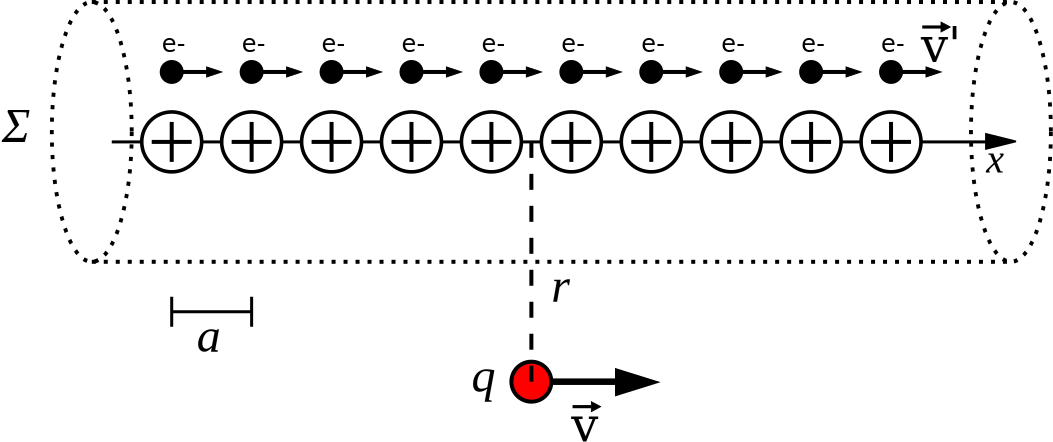
\includegraphics[scale=0.25]{cable.pdf}
\end{figure}

On s'intéresse aux forces électromagnétiques exercées par les charges du fil sur la particule de charge $q$ par deux approches différentes.

\subsubsection*{Approche en mécanique classique}

\begin{itemize}
	\item[$\clubsuit$] Quelle est la densité de charge $\rho_{+}$ (respectivement $\rho_{-}$) due aux atomes (resp. aux électrons) dans le fil ? En déduire le champ électrique $\vec{E}$ créé par cette distribution de charge pour $r>a$.
	
	\item[$\clubsuit$] Quelle est la densité de courant $\vec{j}$ dans le fil ? Exprimer la vitesse $\vec{v'}$ des électrons de conduction en fonction de $I$. En déduire le champ magnétique $\vec{B}$ créé par ce courant en fonction de $v'$ et des autres données de l'énoncé.
	\item[$\clubsuit$] Exprimer la force totale s'exerçant alors sur la charge $+q$, en fonction de $q$, $v$, $v'$, $a$, $r$ et de constantes fondamentales. Quels sont les contributions des forces électriques et magnétiques sur cette particule ?
	\item[$\clubsuit$] Que devient cette force dans le référentiel de la charge $+q$ ? En quoi est-ce une contradiction ?
\end{itemize}

\subsubsection*{Approche en mécanique relativiste}

La théorie de la relativité restreinte permet de lever cette contradiction, en affirmant que tout objet se déplaçant relativement par rapport à un autre voit sa longueur contractée dans le sens du déplacement. Ainsi, Einstein a démontré en 1905 qu'un objet à la vitesse $v$ par rapport à un autre objet, voit la longueur de ce dernier contractée d'un facteur $\gamma(v)=1/\sqrt{1-v^{2}/c^{2}}$ (où $c$ est la vitesse de la lumière). Dans son référentiel, la charge $q$ voit donc la densité de charge des atomes $\rho_+$ et des électrons $\rho_-$ augmenter, mais pas dans les mêmes proportions. 
	\begin{itemize}
		\item[$\clubsuit$] Que deviennent les densités de charge $\rho_{+}$ et $\rho_{-}$ dans le référentiel de la particule $+q$ ? %On admettra que les électrons se déplacent à la vitesse $v'-v$ dans le référentiel de $+q$. 
		\item[$\clubsuit$] Déterminer le champ électrique créé par cette nouvelle distribution de charges en fonction de $v$, $v'$, $a$, $r$ et de constantes fondamentales. On supposera que $v'\ll v\ll c$.
		\item[$\clubsuit$] Quelle est la force électrique s'exerçant sur la particule $+q$ ? 
		\item[$\clubsuit$] Comparer avec le résultat trouvé en approche classique (non relativiste). Que peut-on en dire sur la nature du champ magnétique ?
	\end{itemize}
			
\textit{N.B.} : On rappelle que la vitesse de la lumière $c$ est définie comme $c^{2}=1/\epsilon_{0}\mu_{0}$, où $\epsilon_{0}$ et $\mu_{0}$ sont respectivement la permittivité électrique et la perméabilité magnétique du vide.

\newpage

\section*{Câble coaxial $\bigstar\bigstar$}

On considère un câble coaxial constitué de deux conducteurs cylindriques de même axe, séparés par du vide, de rayon $a$ (l'âme) et $b$ (la gaine), avec $a<b$, et d'épaisseur négligeable. Le conducteur central (de rayon $a$) a une charge surfacique $\sigma_a$ répartie uniformément et est traversé par une densité surfacique de courant $\vec{j_{s,a}}$, répartie aussi uniformément sur l'âme. La longueur du câble est $L$, très grande devant les rayons $a$ et $b$.  

\begin{figure}[h!]
\centering
		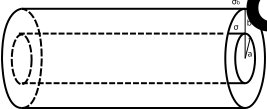
\includegraphics[scale=1]{em2.pdf}
\end{figure}

On cherche à connaitre la capacité et l'inductance linéique du câble coaxial, pour comprendre la propagation des ondes électromagnétiques à l'intérieur. 

\begin{itemize}

	\item[$\blacksquare$] Exprimer le courant $I$ circulant dans l'âme et sa charge totale $Q$ en fonction de $\vec{j_{s,a}}$ et $\sigma_a$. En déduire la charge et l'intensité surfacique de la gaine, $\sigma_b$ et $\vec{j_{s,b}}$, sachant que, sur toute la longueur du câble, le courant total à travers le câble est nul et qu'il est neutre électriquement.
	
	\item[$\blacksquare$] Déterminer le champ électrique en tout point.

	\item[$\blacksquare$] En déduire la capacité $c$ par unité de longueur de câble. 
	
	\item[$\blacksquare$]	 Déterminer le champ magnétique en tout point. 
	
	\item[$\blacksquare$] On définit l'inductance $L$ d'un circuit délimitant une surface $S$, parcouru par un courant $I$ comme  comme le rapport du flux du champ magnétique à travers $S$ avec le courant $I$ :
	\begin{align*}
		\Phi_B=\oiint_S \dif \vec{S}\cdot\vec{B}=LI
	\end{align*}
En choisissant soigneusement une surface $S$, déterminer l'inductance linéique $l$. 

	\item[$\blacksquare$] Que vaut le produit le produit $l\times c$ ? A quoi correspond cette grandeur ?
	
\end{itemize}

\newpage

\section*{Champ magnétique entre deux nappes de courant}

Deux nappes de courant identiques de très grande surface $S = L_x\times L_y$, d’épaisseur $e$, sont parallèles entre elles et séparées d’une longueur $2a$ par un matériau isolant. Elles sont parcourues par un courant permanent de vecteur densité $J\vec{e}_x$ pour la nappe supérieure 1 et $-J\vec{e}_x$ pour la nappe inférieure 2. On se place suffisament loin des bords de la nappe pour négliger les effets de bord.

\begin{figure}[h!]
\centering
		\includegraphics[scale=0.7]{nappe_courant.png}
\end{figure}

\begin{itemize}
	
	\item[$\clubsuit$] Etudier la dépendance et la direction du champ magnétique à partir des symétries et invariances.
	
	\item[$\clubsuit$] Déterminer rigoureusement le champ magnétique dans tous l'espace, et le représenter sur un graphe.
	
\end{itemize}

On définit l'inductance $L$ d'un circuit délimitant une surface $S$, parcouru par un courant $I$ comme  comme le rapport du flux du champ magnétique à travers $S$ avec le courant $I$ :
	\begin{align*}
		\Phi_B=\oiint_S \dif \vec{S}\cdot\vec{B}=LI
	\end{align*}

\begin{itemize}

	\item[$\clubsuit$] Quelle est la surface délimitée par le circuit formé par les deux nappes ? En déduire l'inductance formée par ce système. 
	
\end{itemize}

\newpage

\section*{Champ magnétique dans un cylindre parcouru par un courant orthoradial $\bigstar$}

On considère un cylindre conducteur de rayon $a$ et de longueur $L\gg a$ selon l'axe $O_z$, dans lequel circule une densité volumique de courant $\vec{j}(r)=j_0\vec{e}_\theta$.

\begin{itemize}

	\item[$\circ$] Déterminer l'expression du champ magnétique $\vec{B}(r)$ en fonction de la valeur du champ magnétique en $r=0$.
	\item[$\circ$] Quel est l'expression du champ magnétique $\vec{B}(r)$ si on impose un champ exterieur $\vec{B}_{ext}$ de sorte à ce que  $\vec{B}(r=a)=\vec{0}$ ?

\end{itemize}

\newpage

\section*{Foudre}

On modélise la foudre par un tube d'air ionisé cylindrique de rayon $a$=1m et de densité de courant uniforme $\vec{j}=j_0\vec{e}_z$. Ce sont les électrons de charge $-e$ qui sont supposés porter le courant électrique.

\begin{itemize}

	\item[$\wr$] Sachant que l'intensité d'un éclair peut atteindre 100 kA, quelle est la densité de courant $j_0$ associée ? 

	\item[$\wr$] Etudier la dépendance et la direction du champ magnétique à partir des symétries et invariances.
	
	\item[$\wr$] Déterminer rigoureusement le champ magnétique dans tous l'espace, et le représenter sur un graphe. Estimer la valeur maximale que prend le champ magnétique.
	
	\item[$\wr$] Rappeler l'expression de la force de Lorentz pour un électron de charge $-e$ lorsqu'il est soumis à un champ magnétique extérieur $\vec{B}$. Expliquer succinctement pourquoi le tube d'air ionisé se contracte sur lui-même, se comprimant fortement et générant une grande quantité de chaleur. 

\end{itemize}

\newpage

\section*{Étude d'un colloïde $\bigstar\bigstar$}

Un colloïde est une solution constituée d'un solvant (de l'eau et des ions) et de particules solides en suspension dont la taille peut varier de 10 à 100nm et qui s'ionisent dans le solvant. Par exemple, en agronomie, on étudie les propriétés d'un sol en disolvant un échantillon de terre dans de l'eau. Après traitement, la solution qui en résulte est \textit{une solution colloïdale}, composée des particules d'argile (silice) en suspension dans une eau contenant des ions minéaraux. 

Lorsqu'on augmente la concentration ionique de la solution (en ajoutant du sel par exemple) on observe la sédimentation de la solution colloïdale (les particules d'argiles "tombent" au fond du récipient) : ce phénomène est appelé \textit{floculation} et on cherche à le décrire ici. Il permet notamment de décrire les argiles présente dans la solution.

%Les colloïdes sont constitués par un solvant dans lequel est introduit un corps, généralement solide, qui se disperse sous forme de particules en suspension dont la taille peut varier de 10 à 100nm. Ces particules sont des macromolécules ou des agrégats de petites molécules qui s'ionisent dans le milieu. Par exemple, le blanc d'œuf ou le plasma sanguin sont des solutions colloïdales. En agronomie, le colloïde formé par les particules d'argile (silice) et l'humus (matière organique décomposée) est fondamental pour la fertilité des sols. 

Pour la décrire, on supposera que la solution colloïdale est composée de :
\begin{itemize}
	\item[-] des particules de colloïdes, de rayon $r_0$, portant une charge $Q$ sur leur surface. Ils sont supposés assez dilués pour considérer que le potentiel autour d'une particule colloïdale n'est créée que par elle-même et les ions du milieu ;
	\item[-] les ions contenus dans l'eau à la concentration $N_0$, supposés ponctuels, portant une charge $\pm e$. On supposera que la concentration en cations est égale à celle en anions. Les ions (cations + ou anions -), quand il sont soumis à un potentiel extérieur $V$, se répartissent en moyenne selon la loi de Boltzmann :
\begin{align*}
	\frac{N_{\pm}(r)}{N_0}=\exp\left(-\frac{\pm eV(r)}{k_BT} \right) 
\end{align*}
\end{itemize}
La permitivité du milieu est $\varepsilon=\varepsilon_r\varepsilon_0$ avec $\varepsilon_r=80$. On s'intéresse à une particule de colloïde en suspension dans la solution, entourée d'ions.

%Lorsqu'on augmente significativement la concentration $N_0$ de la solution ionique, on observe que la suspension colloïdale sédimente très rapidement. On cherche à comprendre ce phénomène appelé \textit{floculation}. Pour cela, on s'intéresse à une particule de colloïde en suspension dans la solution, entourée des ions. 

\begin{itemize}

	\item[$\heartsuit$] S'il n'y avait pas d'ions en solution, quel serait le potentiel $V(r)$ autour de la particule de colloïde ? Décrire brièvement comment se répartiraient alors des ions s'ils étaient soumis à ce potentiel.

\end{itemize}

En réalité, la présence de ces ions modifie le potentiel $V$ autour de la particule, qui modifie à son tour la présence d'ions (à travers la densité de charge $\rho$). On souhaite donc trouver deux équations sur $V(r)$ et $\rho(r)$ pour les déterminer. 

\begin{itemize}

	\item[$\heartsuit$] Établir la densité volumique de charge entourant une particule de colloïde. Que devient cette expression si $eV\ll k_BT$ ?
	
	\item[$\heartsuit$] En appliquant le théorème de Gauss, une fois sur une sphère de rayon $r$ autour de la particule, puis une seconde fois en $r+dr$, montrer que : 
	\begin{align*}
		\frac{1}{r^2}\frac{\dif}{\dif r}\left( r^2\frac{\dif V}{\dif r}\right) +\frac{\rho}{\epsilon}=0
	\end{align*}

	\item[$\heartsuit$] Résoudre l'équation différentielle en posant $U(r)=rV(r)$, et retrouver l'expression de $V(r)$, en fonction de $r$, une longueur caractéristique $\lambda$ et une constante d'intégration qu'on ne cherchera pas à définir. Donner un ordre de grandeur de $\lambda$ à température ambiante dans de l'eau pure.
	
	\item[$\heartsuit$] Écrire l'expression du champ électromagnétique. En déduire la constante d'intégration, et l'expression de $V(r)$. 
	
	\item[$\heartsuit$] Quelle est l'expression de la densité de charge $\rho$ ? Justifier l'appellation d'\textit{écrantage}.
	
	\item[$\heartsuit$] Quelle est la force $F(d)$ qui s'exerce entre deux particules de colloïde éloignées d'une distance $d$ ? Comparer cette force dans le cas d'une eau pure et celle d'une électrolyte de concentration $N_0=10^{-7}$mol/L. Pourquoi parle t-on de coagulation ?

\end{itemize} 

\newpage

\section*{Condensateur Terre-ionosphère $\bigstar$}

On représente l'ensemble Terre-ionosphère comme un volumineux condensateur sphérique. La Terre, de rayon $R$, se comporte comme un conducteur parfait de potentiel nul et porte une charge négative $-Q$, uniformément répartie sur sa surface, tandis que la ionosphère est représentée par une surface équipotentielle sphérique de rayon $R+z_0$, de potentiel $V$ possède une charge totale $+Q$. On suppose que la permittivité de l'atmosphère est celle du vide, soit $\varepsilon_0$. 

\begin{figure}[h!]
\centering
		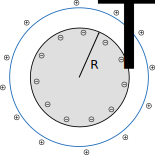
\includegraphics[scale=1]{em3.pdf}
\end{figure}

\begin{itemize}

	\item[$\clubsuit$] Lorsqu'un conducteur parfait est suoumis à un champ électrique extérieur, le champ électrique est nul à l'intérieur de ce conducteur et il se charge en surface. Rappeler pourquoi.
	
	\item[$\clubsuit$] Déterminer le champ électrique $\vec{E}(r)$.
		
	\item[$\clubsuit$] En déduire la capacité $C$ du système Terre-ionosphère.
	
	\item[$\clubsuit$] Des mesures ont permis de déterminer le potentiel de l'ionosphère à l'altitude $z_0=60$km à environ 360kV. Justifier que le système se comporte comme un condensateur plan. Quel est la valeur de la capacité $C$ et l'énergie électrostatique du système $W_{el}$, ainsi que la valeur du champ électrique au niveau du sol.
	
	\item[$\clubsuit$] Donner la valeur de la densité de charge $\sigma$ à la surface de la Terre. Quelle est la charge totale $-Q$ ?
	
	\item[$\clubsuit$] Lors d'un orage, les mouvements convectifs de l'air font passer la tension augmentent fortement la tension entre le sol et le bas des nuages. Les éclairs apparaissent lorsque le champ électrique dépasse un seuil, appelé \textit{champ disruptif} : l'air s'ionise et devient conducteur. Sachant que pour un air humide, ce champ disruptif est de $E_{dis.}\simeq10^{5}$V.m$^{-1}$. A quelle tension $V_1$ observe t-on l'apparition des éclairs ?
	
	
	\textit{Données} : Rayon de la Terre, $R_T=6370$km. Permittivité du vide, $\varepsilon=8,85\cdot10^{-12}$F.m$^{-1}$.
	
\end{itemize}

\newpage

\section*{Condensateur sphère-plan $\bigstar\bigstar\bigstar$}

On considère un conducteur parfait plan, situé en $z=0$ et une sphère de rayon $a$, elle aussi parfaitement conductrice, dont le centre est situé en $(x=0, y=0, z=d)$. La sphère est portée au potentiel $V$ tandis que le plan est relié à la masse, c'est-à-dire u potentiel nul. Le but de l'exercice est de déterminer la capacité entre le plan et la sphère.

\begin{itemize}

	\item[$\circ$] 

\end{itemize}

\newpage

\section*{Exercices en pagaille}

\begin{itemize}

	\item[$\spadesuit$] On considère une boule métallique de rayon $R$. A l'instant $t$, on la monte instantanément au potentiel $V$. Quel est la charge $Q$ de la sphère ? Justifier qualitativement que la charge se répartit sur la surface de la sphère.
	
	\item[$\spadesuit$] On considère un plan infini, avec une charge surfacique $\sigma$. Quel est le champ électrique en tout point de l'espace ? Justifier la présence d'une discontinuité du champ. 
	
	\item[$\spadesuit$] Quel est le champ magnétique créé par une nappe de courant infiniment fine parcouru par une densité de courant $\vec{j_s}$ ? 
	
	\item[$\spadesuit$] A l'aide du théorème d'Ampère, déterminer le champ créé par une bobine de $N$ spires, de longueur $L$ et de rayon $R$, avec $L\gg R$.
	
	\item[$\spadesuit$] On considère un tube parcouru par un courant de densité uniforme $\vec{j}$. Expliquer le phénomène de magnétostriction. On rappelle l'expression de la force de Laplace : $f_{vol}=\vec{j}\dif\tau\wedge\vec{B}$
	
\end{itemize}

\newpage

\section*{Corrosion en phase acqueuse}

\subsubsection*{Corrosion uniforme du zinc en milieu acide}

\begin{itemize}

	\item[$\clubsuit$] Donner l'allure de la courbe densité de courant - potentiel pour l'oxydation et la réduction du couple $Zn/Zn^{2+}$. Ce couple est rapide. Le potentiel standard du couple est -0,76V et on prendra une concentration initiale d'ions zinc II égale à 1 mol.L$^{-1}$.
	
	\item[$\clubsuit$] La courbe intensité-potentiel du couple $H^+/H_2$ dépend-elle du métal utilisé ? Expliquer pourquoi.
	
	\item[$\clubsuit$] On envisage la réduction du zinc par les ions $H^+$. Ecrire l'équation de la réaction. Que peut-on dire de cette oxydation par des considérations thermodynamiques ?

\end{itemize}

Pour des valeurs importantes de la valeur absolue de la densité de courant anodique $\mid j_a\mid$ (resp. cathodique $\mid j_c\mid$), on peut écrire : $j_a=A_a\exp(b_aE)$ et $j_c=-A_c\exp(-b_cE)$. La constante $b_a$ (resp. $b_c$) est positive et caractéristique de l'oxydant (resp. du réducteur). Les constantes $A_a$ et $A_c$ sont positives et dépendent des activités de l'oxydant et du réducteur.

On envisage le phénomène de corrosion uniforme, observée lorsqu'une lame de zinc trempe dans la solution acide. On admet alors que les surfaces d'électrodes sont égales pour l'oxydation et la réduction. 

\begin{itemize}

	\item[$\clubsuit$] Quelle est la relation entre les intensités anodiques et cathodiques ? Que peut-on en déduire sur les densités de courants ?
	
	\item[$\clubsuit$] Une étude expérimentale a permis d'obtenir les lois suivantes, reliant la densité de courant et le potentiel d'électrode mesuré par rapport à l'ESH (les grandeurs sont en unités SI) :
	\begin{itemize}
		\item[-] Oxydation du zinc : $E=0,0774\log_{10}(j_a)-0,1956$
		\item[-] Réduction de $H^+$ sur zinc : $E=-0,0780\log_{10}(\mid j_c\mid)-0,778$
	\end{itemize}
Calculer la densité de courant de corrosion uniforme $j_{corr}$ et le potentiel de corrosion $E_{corr}$.

	\item[$\clubsuit$] La vitesse de corrosion est mesurée en $\mu$m par années. Exprimer littéralement $v_{corr}$ en fonction de $j_{corr}$, de la constante de Faraday $F$, de la masse atomique du zinc et de sa masse volumique. Application numérique : $M_{Zn}=65,4$g.mol$^{-1}$, $\rho_{Zn}=7140$kg.m$^{-3}$ et $F=96490$C.mol$^{-1}$.
\end{itemize}

\subsubsection*{Comparaison avec la corrosion du fer}

\begin{itemize}
	
		\item[$\clubsuit$] On donne $E^0=-0,44$V pour le couple $Fe/Fe^{2+}$. A partir de considérations thermodynamiques, quel métal serait le plus corrodé par la même solution acide ?
		
	\item[$\clubsuit$] Une étude expérimentale, réalisée dans les mêmes conditions, a permis d'obtenir :
	\begin{itemize}
		\item[-] Oxydation du fer : $E=0,0760\log_{10}(j_a)-0,0348$
		\item[-] Réduction de $H^+$ sur fer : $E=-0,0780\log_{10}(\mid j_c\mid)-0,476$
	\end{itemize}
	Calculer la densité de courant de corrosion uniforme du fer et conclure.
		
	\item[$\clubsuit$] Représenter grossièrement les graphes $E(\log j)$ pour l'oxydation du zinc, la réduction de $H^+$ sur zinc, l'oxydation du fer, la réduction de $H^+$ sur fer. On se limitera aux valeurs de $E$ comprises entre 0 et-1V et de $\log j$ comprises entre 0 et -5.
	
	\item[$\clubsuit$] Deux blocs, l'un de fer et l'autre de zinc de même surface et reliés électriquement, sont plongés dans la solution acide précédente. Décrire les phénomènes observés, indiquer quel métal sera le plus corrodé et calculer la densité de courant. Conclure. 
	
\end{itemize}

\end{document}
